\documentclass[final]{beamer}
\usetheme{NTH}
\usepackage[orientation=portrait,size=a1,scale=1.4,debug]{beamerposter}
\usepackage[absolute,overlay]{textpos}
\usepackage{graphicx}
\usepackage{multicol}
\usepackage{siunitx}
\setlength{\TPHorizModule}{1cm}
\setlength{\TPVertModule}{1cm}

\title{Modelling the effects of domestication in Wheat through novel computer-vision techniques}
\author{Nathan Hughes (nah26@aber.ac.uk)}
\footer{More information at \texttt{http://www.users.aber.ac.uk/nah26}}
\date{\today}

\begin{document}
\begin{frame}{}

  \begin{textblock}{28}(1,5.5)

    \begin{block}{Introduction}


      My Project's goal is to examine the effects of domestication in Wheat through the use of \si\micro\-Computed Tomography.
      This will be done by using a novel technique for a detailed extraction of 3-dimensional morphometric data of wheat grain \cite{hughes2017}.

      \vspace{0.5cm}

      I have a wide range or primitive, non-domesticated wheat varieties
      as well as their cultivated relatives. These genotypes also provide a nice gradient of genome shape and size (Ploidy)
      which could also provide great insight into how genome structure effects grains.

      \vspace{0.5cm}

      I aim to modify, improve and use the outlined method to extract data from these wheat varieties to create a unique data-set.
      I shall then create statistical analysis software which can reliably, produce answers to hypothesis aimed at these data.

    \end{block}


    \begin{block}{Grain Parameters}

      The technique being used to produce these data provides a number of attributes for me to use in
      analysis. The primary ones can be seen in the figure \ref{fig:real}

      \begin{multicols}{2}
        \begin{figure}[htb]
          \centering
          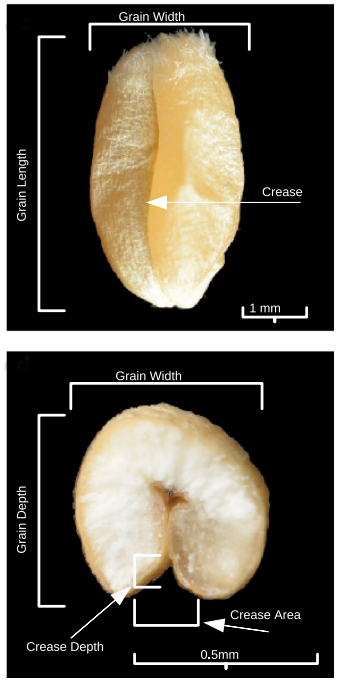
\includegraphics[width=7.3cm]{collection2.png}
          \caption{\label{fig:real} wheat grains labelled with data}
        \end{figure}

        \columnbreak

        \begin{figure}[htb]
          \centering
          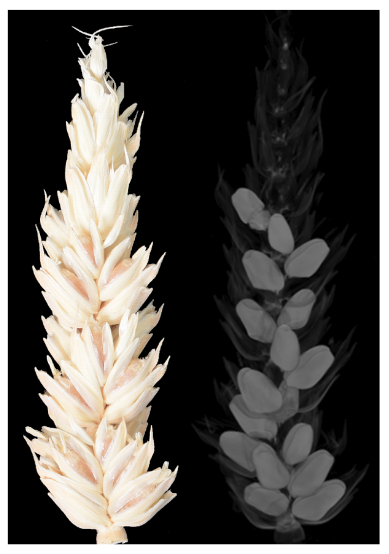
\includegraphics[width=10.5cm]{collection.png}
          \caption{\label{fig:3d} wheat Spikes original (left) and scanned (right)}
        \end{figure}

      \end{multicols}

    \end{block}

    \begin{block}{Software Development and Pipeline}
      \begin{multicols}{2}

      To make this research reproducible, for use in follow-up and future experiment analysis,
      I am creating a software library which acts as a specialist pipeline for handling CT-Scanner
      image data.

      \vspace{0.5cm}

      Figure:\ref{fig:flow} Illustrates a typical pipeline in which data will flow in this system.
      Primarily the process aims at taking raw uninteresting data and producing meaningful and useful
      output.

      \vspace{0.5cm}

      The pipeline will also allow a researcher to specify if they are interested in cleaning the data
      or if the outliers are of particular interest, additional options for joining in other external
      experiment information will also be possible in the final design, as flexibility is key.

        \columnbreak

        \begin{figure}[htb]
          \centering
          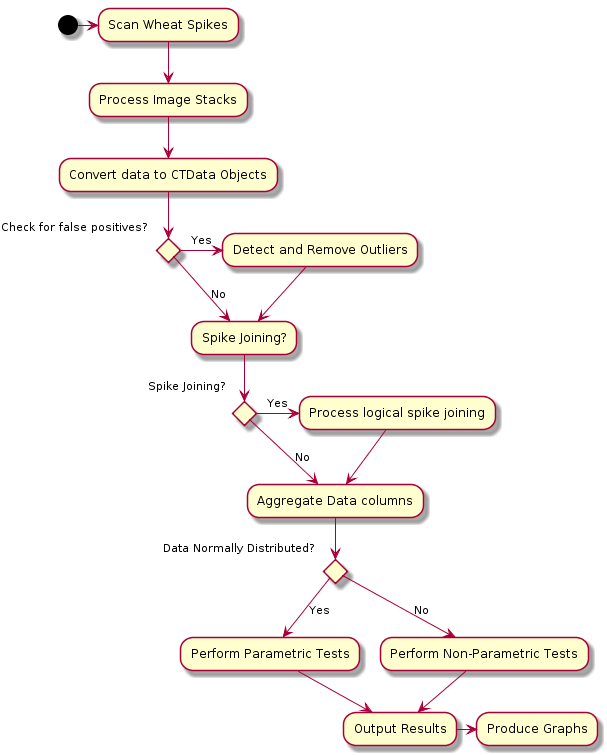
\includegraphics[width=13.5cm, height=20cm]{flow.png}
          \caption{\label{fig:flow} Data Processing Software Pipeline }
        \end{figure}

      \end{multicols}




    \end{block}

    \begin{block}{Future Work}
      My main aim for the future is to fully implement the proposed statistical library,
      once completed I can focus on testing my outlined hypothesis.
      I will also be aiming to make use of the \textit{scipy}
      data models packages in Python.
    \end{block}


    \begin{block}{Further Information}
      For more information on this project I recommend keeping up-to-date with my development blog
      which can be found at  http://www.users.aber.ac.uk/nah26

      Also with Dr. Hugo Oliveira's work which can be found on Google scholar
      provides a great deal of insight into the primitive species
      and their phylogeny.

    \end{block}


  \end{textblock}

  \begin{textblock}{28}(30.5,5.5)

    \begin{block}{Research Aims}
      Primarily I have three main null-hypothesis which I hope this project will be able to reject:

      \begin{itemize}
      \item{$H_0=$ Domestication has no effect on the morphometric properties of wheat}
      \item{$H_0=$ Ploidy has no effect on the morphometric properties of wheat}
      \item{$H_0=$ There is no difference in hulled and non-hulled genotypes}
      \end{itemize}

    \end{block}


    \begin{block}{Current Progress}

      My work to date has been primarily focused on modifying
      and adapting 3D analysis software to fit the required
      parameters to work with such a varied data source.

      \vspace{0.3cm}

      Additionally I have been building a data processing library whichs aims to:
      \begin{multicols}{2}

        \begin{itemize}
        \item simplify data input
        \item perform data cleaning
        \item automatically generates plots
        \end{itemize}
        \columnbreak
        \begin{itemize}
        \item handles data from multiple sources
        \item adding additional experiment parameters
        \end{itemize}

      \end{multicols}

      \vspace{0.3cm}

      Figure \ref{fig:initalboxplots} shows one example of the auto analysis which my library
      can perform in its early stages of development.

      \begin{figure}[htb]
        \centering
        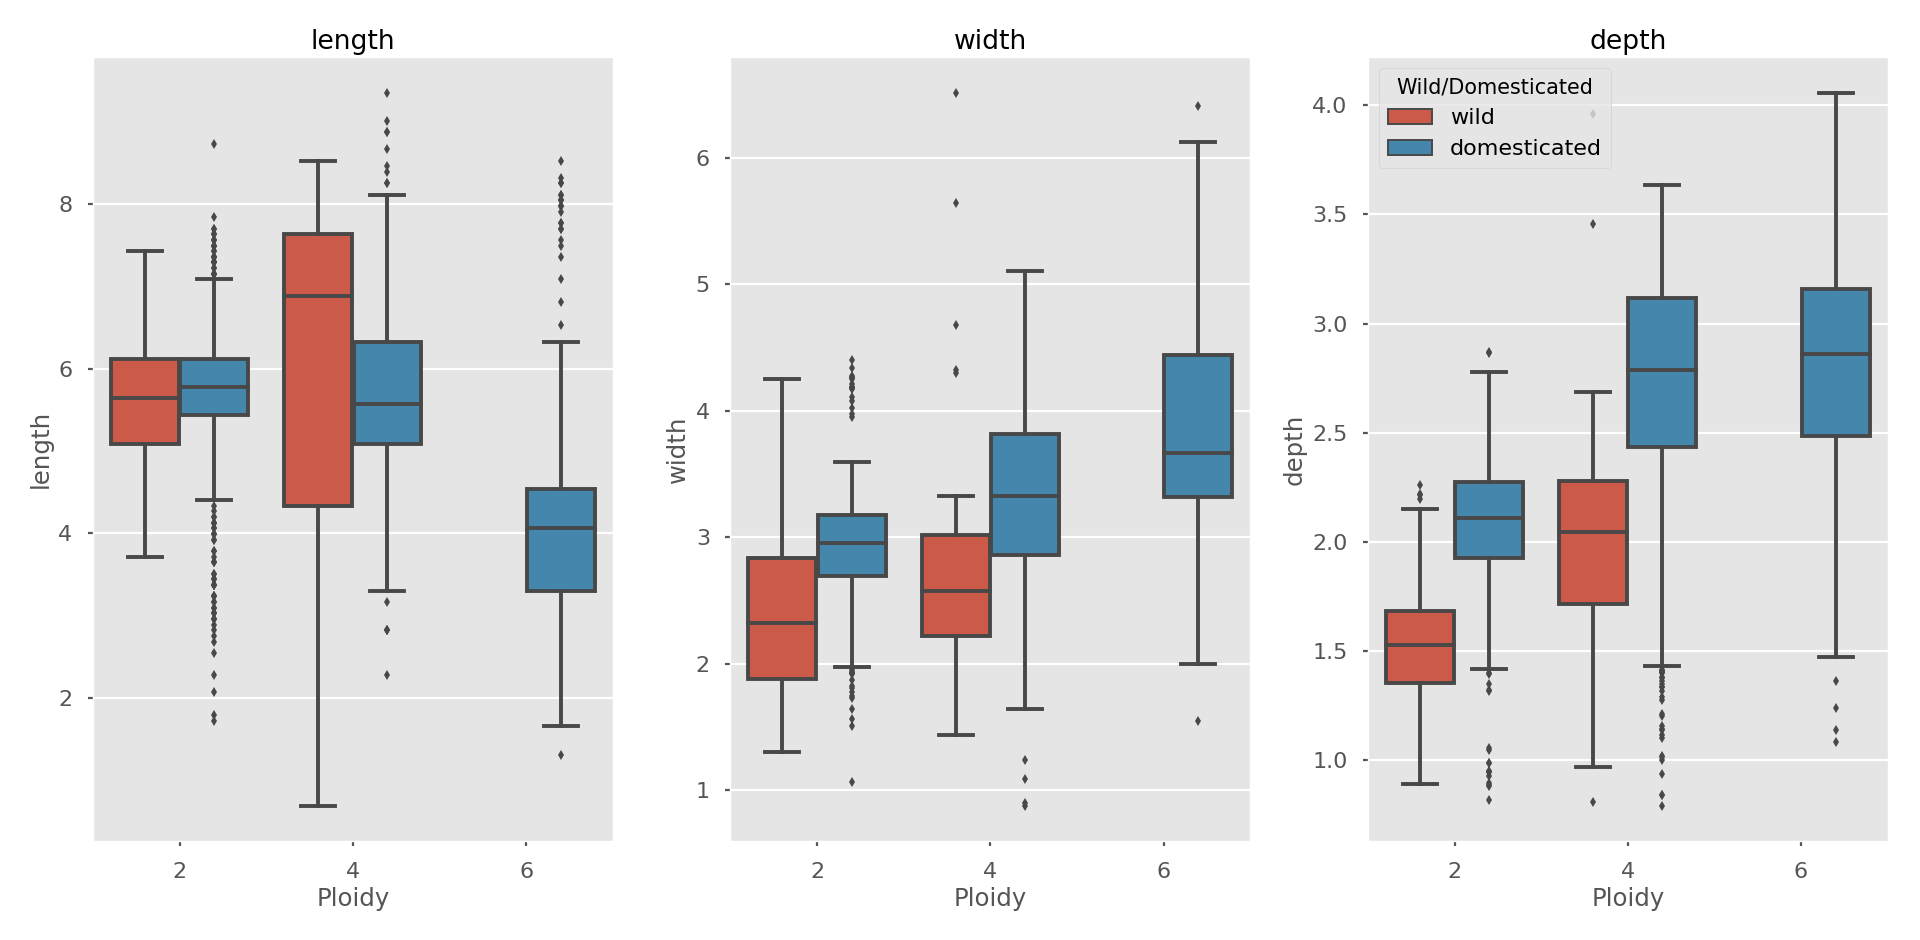
\includegraphics[width=22cm]{domesticated.png}
        \caption{\label{fig:initalboxplots}Initial Data analysis of Domestication and Ploidy}
      \end{figure}

    \end{block}


    \begin{block}{Statistical Methods and Testing}

      In order to answer these questions a number of statistical tests will be required,
      as will numerous elements of data science, all of which will be incorporated into
      my analysing software library (Figure:\ref{fig:flow}). I am planning to use:

      \begin{multicols}{2}

        \begin{itemize}
        \item ANOVA
        \item MANOVA
        \item $\chi^2$ Tests
        \end{itemize}

        \columnbreak

        \begin{itemize}
        \item PCA
        \item GLMs
        \item T/F-Tests
        \end{itemize}

      \end{multicols}

      From the data in Figure:\ref{fig:initalboxplots} you can see that the data is
      messy before processing. I have used QQ-Plots in Figure:\ref{fig:qq} to illustrate
      the non-parametric nature of the data. This is a problem I hope to solve in the future.
        \begin{figure}[htb]
          \centering
          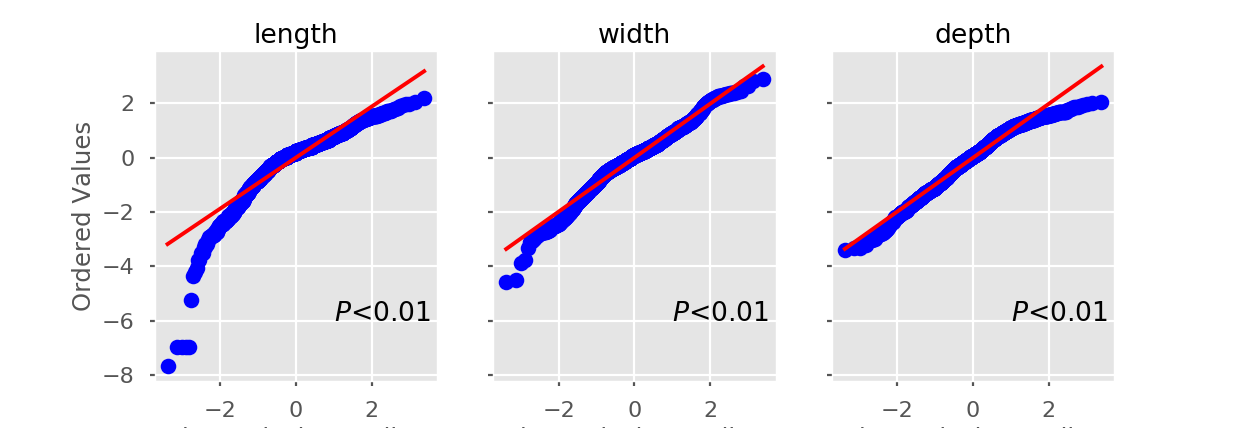
\includegraphics[width=22cm]{qqplots.png}
          \caption{\label{fig:qq} QQ-Plots showing Distribution}
        \end{figure}

    \end{block}


    \begin{block}{Acknowledgements and Thanks}
      Thank you for the vital help and support from the following people and organisations.

      \begin{multicols}{3}

        \begin{itemize}
        \item{Dr. Wayne Aubrey}
        \item{Dr. Candida Nibau}

        \end{itemize}

        \columnbreak

        \begin{itemize}
        \item{Prof. John Doonan}
        \item{Dr. Hugo Oliveira}

        \end{itemize}

        \columnbreak

        \begin{itemize}
        \item{BBSRC}
        \item{Dr. Kevin Williams}
        \end{itemize}

      \end{multicols}

    \end{block}

    \begin{block}{References}
      \bibliography{poster}
      \bibliographystyle{unsrt}
    \end{block}


  \end{textblock}

\end{frame}
\end{document}

%%% Local Variables:
%%% mode: latex
%%% TeX-master: t
%%% End:
